\section{Introduction}
When considering the 100 years of the 20th century in popular music including jazz, it can be said that ``{\bf the 20th century was a hundred years in which music born in the southern United States spread around the world in various forms}''\cite{murai:01}. It goes without saying that this development began with sheet music in the early days and was disseminated through the invention of radio, records, and mass media. However, why is there a predominance of common time signatures such as 4/4 or 3/4 in much of this music's rhythm? The author believes that even in modern times, the system for describing music—``the musical score as a protocol connecting composers and performers''—inherited from classical music has a strong influence on music theory such as the Berklee Method and modern music production environments.

On the other hand, many attempts have been made to depart from existing rhythmic forms in contemporary music, free jazz, noise music, and electronica. However, most of these have been included as partial elements in modern popular music without changing or updating the rhythmic forms themselves.

Therefore, focusing on approaches to jazz rhythm in the modern era from around the 21st century, such as ``polyrhythm/cross-rhythm characteristics'' and ``fluctuations and inflections in rhythm,'' and expanding these methods as a critical attempt toward 20th-century music, the author devised ``music with multilayered temporal structures.'' As a practical example, a series of works titled ''{\bf Music for multilayered temporal structures}''\cite{yamato:01} was composed, and performances by jazz musicians were attempted and recorded to examine whether actual performance was possible.

\subsection{Scope of This Research \label{research_target}}
As stated in the introduction, this research presents a critical perspective on the rhythmic forms of current popular music, as well as production environments such as notation and DTM, from the viewpoint of ``possibilities for future rhythmic approaches.'' Regarding why such a critical attempt is necessary, Yuval Noah Harari states in \textit{Sapiens: A Brief History of Humankind}:\\

{\bf Just as medieval culture could not reconcile chivalry with Christianity, so the modern world fails to reconcile liberty with equality. But this is no defect. Such contradictions are an inseparable part of every human culture. In fact, they are culture's engines, responsible for the creativity and dynamism of our species. Just as when two clashing musical notes played together force a piece of music forward, so discord in our thoughts, ideas and values compels us to think, reevaluate and criticize. Consistency is the playground of dull minds.
If tensions, conflicts, and irresolvable dilemmas are the spice of every culture, a human being who belongs to any particular culture must hold contradictory beliefs and be riven by incompatible values. It's such an essential feature of any culture that it even has a name: cognitive dissonance. Cognitive dissonance is often considered a failure of the human psyche. In fact, it is a vital asset. Had people been unable to hold contradictory beliefs and values, it would probably have been impossible to establish and maintain any human culture.} \cite{harari:01}\\

The ``dissonance'' that Harari mentions here is clearly not musical dissonance but a metaphor. However, as shown in Figure \ref{fig:figure_08}\cite{murai:01}, the collision between African music and Irish music of Islamic origin within Creole culture, which became one of the origins of jazz and had a major influence on today's popular music and was also the impetus for the birth of blues music, can also be described as the ``cognitive dissonance for humanity to establish culture'' that Harari refers to. It can also be considered that such cognitive dissonance has occurred in various forms to this day, maintaining and developing culture as popular music.

\begin{figure}[ht]
\centerline{
	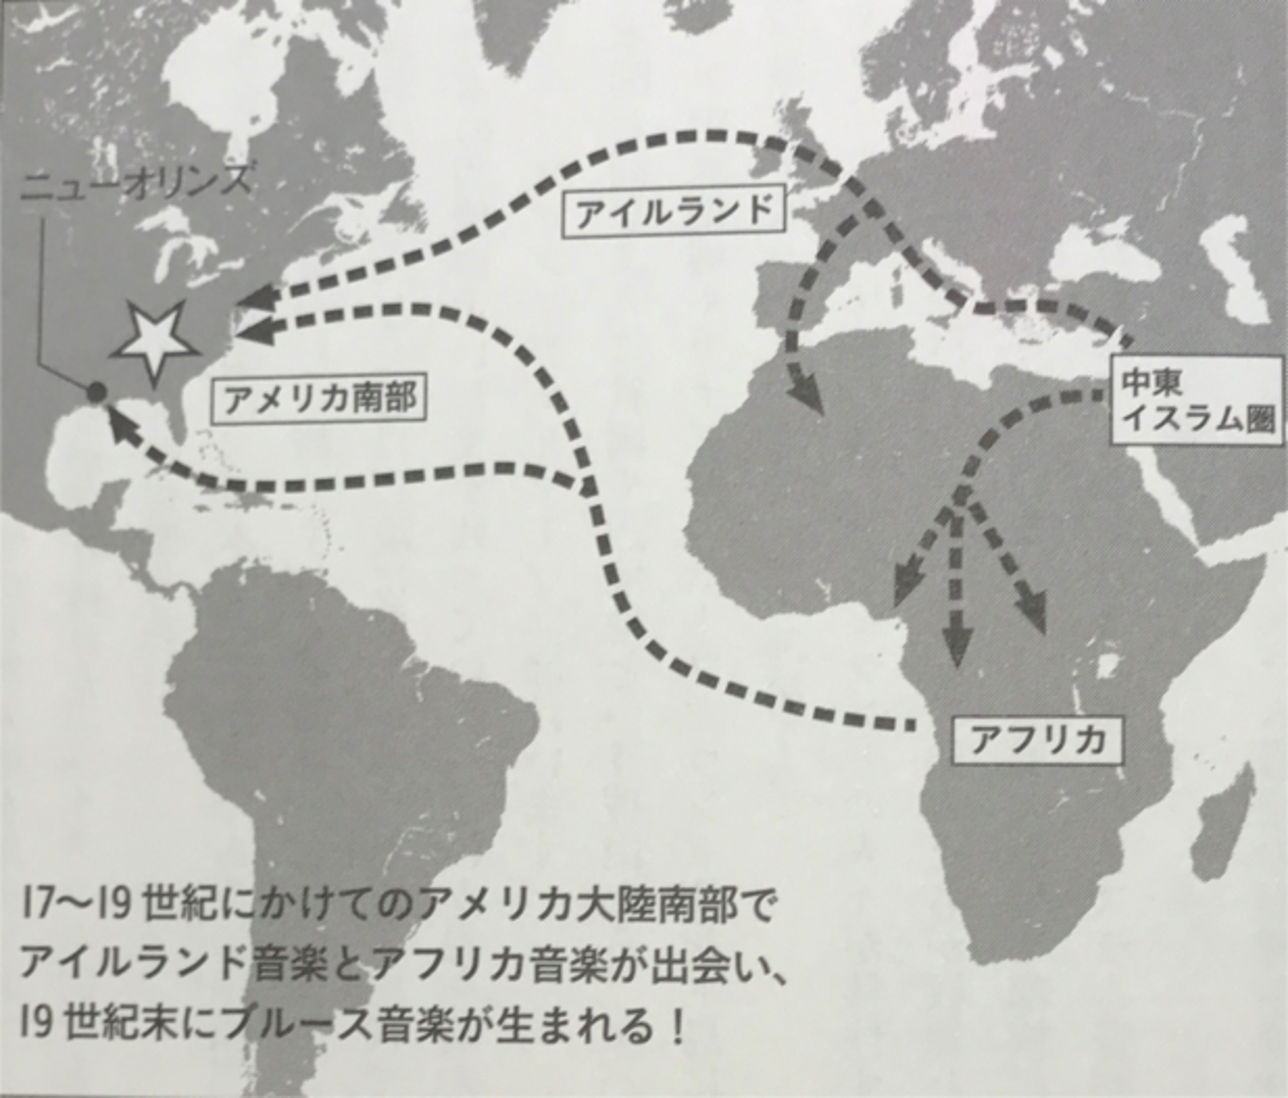
\includegraphics[
 width=0.5\textwidth]{./PDF/figure_08.pdf}
}
\caption{Mukai Yasushi (\textit{Jazz History That Changes Your Listening}, p17, 2017)\\
A diagram showing the origin of blues, where music from the Middle Eastern Islamic region influenced and passed through African music and Irish music, then converged in the southern United States}
\label{fig:figure_08}
\end{figure}

Furthermore, the purpose of this research is to carry out the movement from dissonance to harmony that Harari describes through ``approaches to rhythm,'' prompting listeners, performers, and composers to reevaluate, criticize, and critique, thereby creating ``cognitive dissonance through rhythm'' and contributing to advancing music as a culture.

To this end, this research and the works produced in the process will be discussed primarily within the context of popular music. Specifically, through the development of the Berklee Method, which formed the foundation of popular music, and the creation of jazz-based works using lead sheet notation, which is one of the reasons for the worldwide spread of this theory, this research will address approaches to rhythm, notation methods, and performance feasibility.


\subsection{Similarities Between Modern Popular Music History and Western Music History}

This research examines so-called ``popular music,'' and its background will be discussed here. First, when proceeding with the argument on the two axes of ``Western music'' and ``popular music'' in this section, each will be defined as follows.

\begin{description}
 \item[Western music]\mbox{}\\
	    Refers mainly to classical music and contemporary music before the 20th century. Also includes music from the 20th century onward that follows this style.
 \item[Popular music]\mbox{}\\
	    Refers mainly to music based on blues and jazz as American ethnic music from the 20th century onward. Includes commercial music in general.
\end{description}

As the basis for such a division, Peter van der Merwe states in \textit{Origins of the Popular Style}: ``{\bf By the time the first blues was published, all the materials available to twentieth-century popular music composers were in place. Since then, popular music has incorporated various ethnic styles, drawn inspiration from classical music, and combined the styles at hand in every possible way. (omitted) But fundamentally speaking, no elements have been created whose origins do not date back to before the 1900s}'' \cite{merwe:01}. However, at the same time, Merwe also states: ``{\bf The term `popular music' is a label, not a content. (omitted) Being popular, whether it means `favored by the people' or `of the masses,' is only a temporary value}'' \cite{merwe:01}. This indicates that the two definitions divided above are merely a convenient division based on historical background and do not indicate their value.

Assuming such a division is possible, what is important here is Merwe's earlier observation that ``no elements have been created whose origins do not date back to before the 1900s.'' This demonstrates the self-evidence that ``popular music'' contains within it the context of ``Western music,'' but the author attempts to present both the similarities and what ``Western music'' has overlooked, as well as the present state of ``popular music,'' by placing ``Western music'' and ``popular music'' in parallel based on their developmental history.

First, when considering ``Western music'' as the flow from so-called ``classical music to contemporary music (including American New Music such as John Cage and Steve Reich),'' we can broadly understand it as the establishment of tonality in the Baroque period from the 17th to 18th centuries, the Romantic period and popularization from opera to aria in the 19th century, and the flow to contemporary music through the expansion of tonality from twelve-tone technique and serialism in the 20th century. When comparing ``popular music'' with the flow toward blues and jazz as American ethnic music, the diversification and theorization of styles such as the ``popular music theory'' born there—the Berklee Method, modal jazz, and free jazz—followed by mass production and media distribution and development of pop music leading to popularization, and the expansion of diversity through electronics, both can be seen to follow a flow of ``establishment of tonality, expansion, and atonality.'' In particular, the chord system spread by the Berklee Method after entering the 20th century and the high analytical nature of that system greatly changed the production field from before its appearance, and it can be said that ``{\bf the Berklee Method represents the first peak of symbolization in the history of `commercial music,' probably in a history that will continue for a long time to come}'' \cite{kikuchi-ootani:01}. This can also be described as ``{\bf symbolization = commercialization = emphasis on phonemes}'' \cite{kikuchi-ootani:01}, similar to the flow of ``establishment of tonality to popularization'' in Western music. Also, if we place the movement from ``expansion of tonality to contemporary music'' in ``Western music'' in parallel with ``mode, free, noise as methods, and the development and diversity of technology/electronics'' in ``popular music,'' both can be understood as a movement of ``expansion of tonality to atonality.'' By understanding both in parallel in this way, it can be said that much of the flow of ``establishment of system,'' ``expansion of system,'' and ``departure from system'' is being carried out by both centered on ``tonality.'' Furthermore, by understanding modern ``popular music'' from this standpoint, it becomes possible to consider the possibilities of future music.

